\documentclass[border=3mm,tikz,preview]{standalone}
\usepackage[utf8]{inputenc}
\usepackage{amsmath,amssymb,amsfonts}
\usepackage{graphicx}
\usepackage{tikz}
\usetikzlibrary{shapes.geometric, arrows.meta, positioning, shadows, calc, fit, backgrounds}
\usepackage{xcolor}
\begin{document}

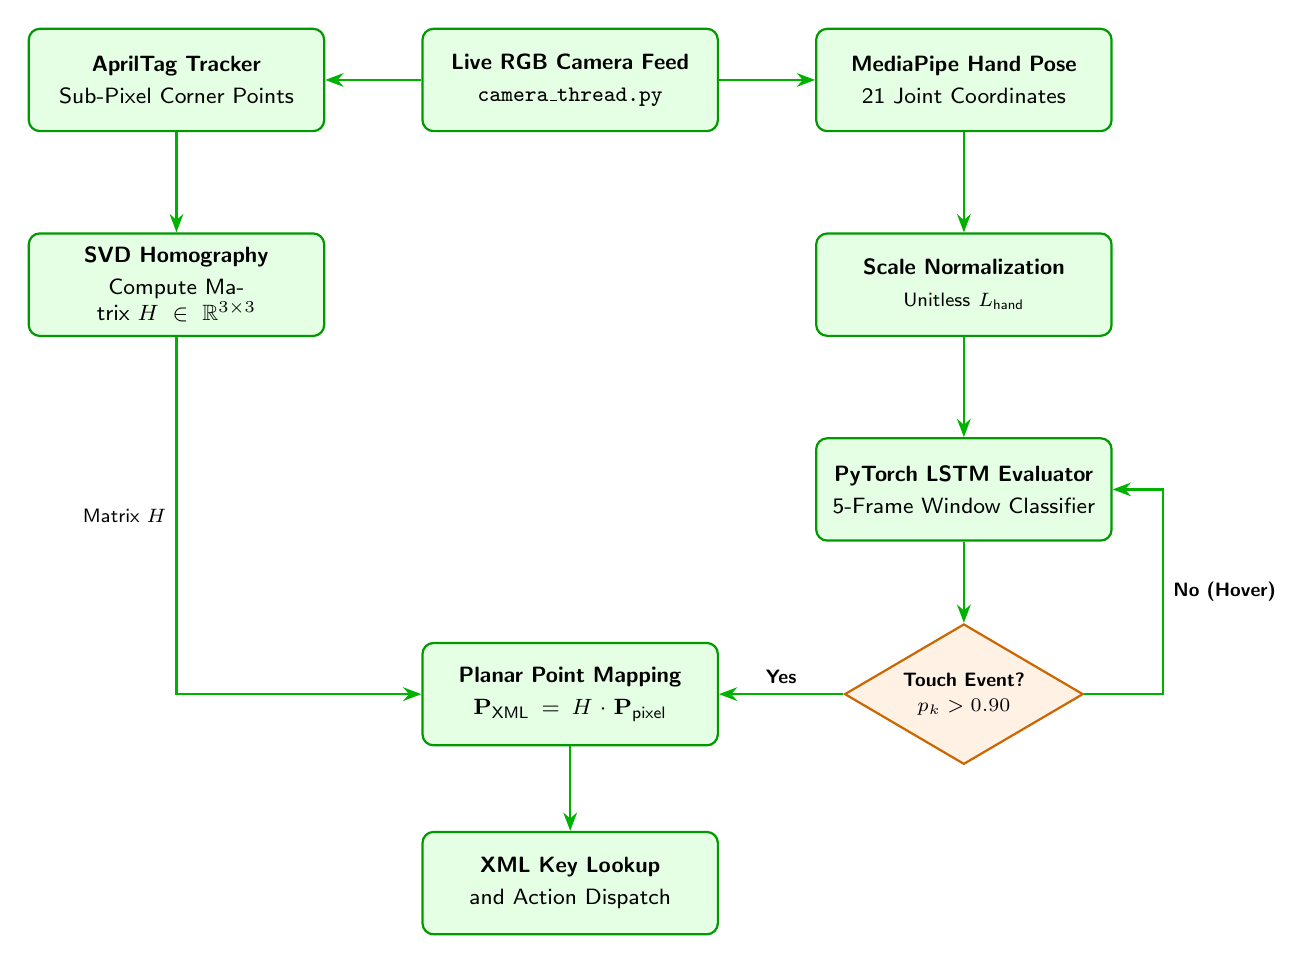
\begin{tikzpicture}[
    block/.style = {rectangle, draw=green!60!black, fill=green!10!white, thick, rounded corners=4pt, align=center, font=\sffamily\footnotesize, text width=3.4cm, minimum height=1.3cm, inner sep=5pt},
    decision/.style = {diamond, draw=orange!80!black, fill=orange!10!white, thick, align=center, font=\sffamily\scriptsize, inner sep=3pt, aspect=1.7},
    arrow/.style = {draw=green!70!black, ->, >=Stealth, thick}
]

% Row 1 (y = 0): Camera Feed in Center (x = 5.0), branching Left (x = 0) and Right (x = 10.0)
\node (cam) [block] at (5.0, 0) {\textbf{Live RGB Camera Feed}\\[2pt]\texttt{camera\_thread.py}};
\node (april) [block] at (0, 0) {\textbf{AprilTag Tracker}\\[2pt]Sub-Pixel Corner Points};
\node (mp) [block] at (10.0, 0) {\textbf{MediaPipe Hand Pose}\\[2pt]21 Joint Coordinates};

% Row 2 (y = -2.6): Left = Homography, Right = Scale Normalization (Center is open)
\node (homog) [block] at (0, -2.6) {\textbf{SVD Homography}\\[2pt]Compute Matrix $H \in \mathbb{R}^{3 \times 3}$};
\node (norm) [block] at (10.0, -2.6) {\textbf{Scale Normalization}\\[2pt]{\scriptsize Unitless $L_{\text{hand}}$}};

% Row 3 (y = -5.2): Right = PyTorch LSTM Evaluator
\node (lstm) [block] at (10.0, -5.2) {\textbf{PyTorch LSTM Evaluator}\\[2pt]5-Frame Window Classifier};

% Row 4 (y = -7.8): Left/Center = Coordinate Mapping, Right = Touch Decision Diamond
\node (map_coord) [block] at (5.0, -7.8) {\textbf{Planar Point Mapping}\\[2pt]$\mathbf{P}_{\text{XML}} = H \cdot \mathbf{P}_{\text{pixel}}$};
\node (touch_dec) [decision] at (10.0, -7.8) {\textbf{Touch Event?}\\[1pt]{\scriptsize $p_k > 0.90$}};

% Row 5 (y = -10.2): Center = XML Key Lookup & Dispatch
\node (lookup) [block] at (5.0, -10.2) {\textbf{XML Key Lookup}\\[2pt]and Action Dispatch};

% Connections: Camera Distribution
\draw [arrow] (cam.west) -- (april.east);
\draw [arrow] (cam.east) -- (mp.west);

% Left Track: AprilTag to Homography
\draw [arrow] (april.south) -- (homog.north);

% Right Track: MediaPipe to Normalization to LSTM to Decision
\draw [arrow] (mp.south) -- (norm.north);
\draw [arrow] (norm.south) -- (lstm.north);
\draw [arrow] (lstm.south) -- (touch_dec.north);

% Hover Loop (routes cleanly around right side of LSTM)
\draw [arrow] (touch_dec.east) -- ++(1.0, 0) |- node[near start,right,font=\sffamily\scriptsize]{\textbf{No (Hover)}} (lstm.east);

% Touch Confirmed (generous 1.8cm clearance between boxes)
\draw [arrow] (touch_dec.west) -- node[above,font=\sffamily\scriptsize]{\textbf{Yes}} (map_coord.east);

% Homography Matrix Feed (drops vertically through open space, then turns into map_coord)
\draw [arrow] (homog.south) |- node[near start,left,font=\sffamily\scriptsize]{Matrix $H$} (map_coord.west);

% Dispatch Execution (straight vertical arrow down)
\draw [arrow] (map_coord.south) -- (lookup.north);

\end{tikzpicture}

\end{document}
